\def\find{\mathop{\mathit{find}}}
\def\delete{\mathop{\mathit{delete}}}

\subsection{\emph{d}-árna halda} 
\paragraph{Popis.}
Ako zovšeobecnenie binárnej haldy môžeme považovať $d$-árnu haldu. Rozdiel je v stupni vrcholov:
%Každý vrchol v binárnej halde okrem listov má stupeň 2, v d-árnej halde je stupeň vrcholov $d$.
$d$-árna halda je, až na poslednú úroveň, \emph{úplný $d$-árny strom} spĺňajúci podmienku haldy. Posledná úroveň je 
\emph{zľava úplná}.
Halda sa najčastejšie reprezentuje v poli, koreň je na mieste $0$ a synovia $i$-teho prvku sú v poli na miestach 
$(d\cdot i + 1)$ až $(d\cdot i + d)$.
%V našej implementácií navyše každý vrchol obsahuje smerník na svojho otca a smerník na pole synov.
S takouto reprezentáciou v poli "zľava úplný" $d$-árny strom znamená, že v poli, v ktorom je uložený, nie sú "diery". 

\begin{figure}
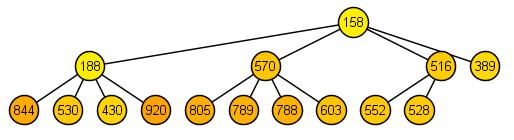
\includegraphics[width=\columnwidth]{obrazky/daryheap.png}
\caption{\emph{Príklad $d$-árnej haldy pre $d = 4$.} Vrcholy s menším kľúčom majú svetlejšiu farbu.} 
\label{img:komp} 
\end{figure}

\paragraph{Operácie.}
Operácia $\ins(x)$ vloží vrchol s kľúčom $x$ na najbližšie voľné miesto, tak, aby sa neporušila úplnosť stromu 
a poslednej vrstvy. V praxi to znamená, že sa pridá nový prvok na koniec poľa. Takto vložený prvok môže porušovať 
podmienku haldy, takže ešte musí "prebublať" smerom hore na správne miesto. Vymieňa sa so svojím otcom, až pokým 
nie je podmienka haldy splnená.

Minimum sa nachádza v koreni haldy. Operácia \emph{deleteMin} najprv vymení koreň haldy s posledným vrcholom a potom 
minimum, ktoré sa teraz nachádza na konci haldy, odstráni. Koreň haldy po výmene nemusí spĺňať podmienku haldy a 
preto musí "prebublať" nadol. Vymieňa sa so svojím najmenším synom, až pokým nie je splnená podmienka.

Po zavolaní operácie $\dec(v, \Delta)$ vrchol $v$ nemusí spĺňať podmienku haldy a preto musí opäť 
"prebublať" nahor.

\paragraph{Časová zložitosť.}
Z popisu jednotlivých operácií sú zrejmé časové zložitosti:
Ak $n$ je počet prvkov v halde, potom operácie $\ins$ a $\dec$ majú časovú zložitosť $O(\log_d(n))$, pretože 
$\log_d(n)$ je hĺbka stromu, teda vrchol sa po $\log_d(n)$ krokoch dostane ku koreňu. Operácia \emph{deleteMin} má 
zložitosť $O(d\cdot \log_d(n))$, pretože sa navyše pri prebublávaní musí hľadať najmenší syn spomedzi $d$ synov;
$\mathit{findMin}$ sa deje v konštantnom čase.

\paragraph{Použitie.}
Z časových zložitostí platiacich pre binárnu haldu sa môže zdať vznik $d$-árnej haldy zbytočný. Avšak v mnohých 
reálnych prípadoch funguje zovšeobecnená verzia efektívnejšie, najmä ak sú operácie $\ins$ a $\dec$
využívané častejšie ako operácia \emph{deleteMin}. Ak napríklad v Dijkstrovom, či Jarníkovom--Primovom
algoritme zvolíme $d=m/n$, vieme nájsť najkratšiu cestu, resp.\ minimálnu kostru v čase $O(m\log_{m/n} n)$.

Pre malé $d>2$ funguje $d$-árna halda rýchlejšie než binárna vďaka lepšej práci s rýchlou vyrovnávacou pamäťou
(cache); veľké $d$ sú vhodné pre dátovú štruktúru uloženú na disku (kde sa počet prístupov na disk snažíme minimalizovať,
podobne ako pri B-strome).

